\documentclass[10pt, aspectratio=169]{beamer}

\usepackage[utf8]{inputenc}
\usepackage[T1]{fontenc}
\usepackage[ngerman,shorthands=off]{babel}
\usepackage{graphicx}
\usepackage[absolute,overlay]{textpos}
\usetheme{Madrid}
\usecolortheme{seahorse} 
\setbeamertemplate{navigation symbols}{}
\usepackage[backend=biber]{biblatex}
\addbibresource{/Users/jakubmarczak/Downloads/literatur.bib}
\usepackage{csquotes}
\usepackage{hyperref}
\usepackage{wasysym}
\usepackage{xcolor}
\usepackage{tikz}
\definecolor{progress}{HTML}{9b9bba}
\usepackage{listings}
\usepackage{xcolor}

\lstset{
  language=R,
  basicstyle=\ttfamily\small,
  keywordstyle=\color{blue},
  commentstyle=\color{gray},
  stringstyle=\color{red},
  showstringspaces=false,
  breaklines=true
}

\title{Projekt \MakeUppercase{\romannumeral 1}  Zwischenpräsentation}
\author[J. Marczak, G. Kathiravan, M. I. Rahman]{Jakub Marczak, Ganeisraaj Kathiravan, Muhammad Ibrahim Rahman}

\setbeamertemplate{footline}{
  \leavevmode
  
  % Infoleiste
  \hbox{
    \begin{beamercolorbox}[wd=.333333\paperwidth,ht=2.5ex,dp=1ex,left]{author in head/foot}
      \hspace{1em}\insertshortauthor
    \end{beamercolorbox}
    \begin{beamercolorbox}[wd=.333333\paperwidth,ht=2.5ex,dp=1ex,center]{title in head/foot}
      \insertshorttitle
    \end{beamercolorbox}
    \begin{beamercolorbox}[wd=.333333\paperwidth,ht=2.5ex,dp=1ex,right]{date in head/foot}
      \insertframenumber{} / \inserttotalframenumber \hspace{1em}
    \end{beamercolorbox}
  }

  % Progressbar
  \hbox{
    \begin{beamercolorbox}[wd=\paperwidth,ht=1.3ex,dp=0ex,left]{}
      \tikz{
        \fill[gray!15] (0,0) rectangle (\paperwidth,1.3ex);
        \fill[progress] (0,0) rectangle
        ({\paperwidth*\insertframenumber/\inserttotalframenumber},1.3ex);
      }
    \end{beamercolorbox}
  }
}

\begin{document}

\begin{frame}[plain]
  \titlepage
\end{frame}

% Folie 2
\begin{frame}
    \frametitle{Inhalt}
    \begin{enumerate}
        \item Datensatz \& Methoden
        \item Zentrale Ergebnisse
        \begin{itemize}
            \item Unterschiede zwischen Ost- und Westdeutschland
            \item Prädiktoren für Arbeitslosigkeit
        \end{itemize}
    \end{enumerate}
\end{frame}

% Folie 3 
\begin{frame}[fragile]{R Code Beispiel}
    \frametitle{Datensatz \& Methoden}
%    \begin{figure}
%        \centering
%        \includegraphics[width=1\linewidth]{population.pdf}
%        \vspace{-0.75cm}
%        \caption{Kerndichteschätzungen mit Gaußkern für Alter, Größe und Gewicht.}
%    \end{figure}
        \begin{itemize}
            \item Behandelte Variablen
        \end{itemize}
        \begin{itemize}
            \item Benutzte Methoden
        \end{itemize}
\end{frame}

% Folie 4 
\begin{frame}[fragile]{R Code Beispiel}
    \frametitle{Zentrale Ergebnisse}
    \begin{figure}
        \centering
        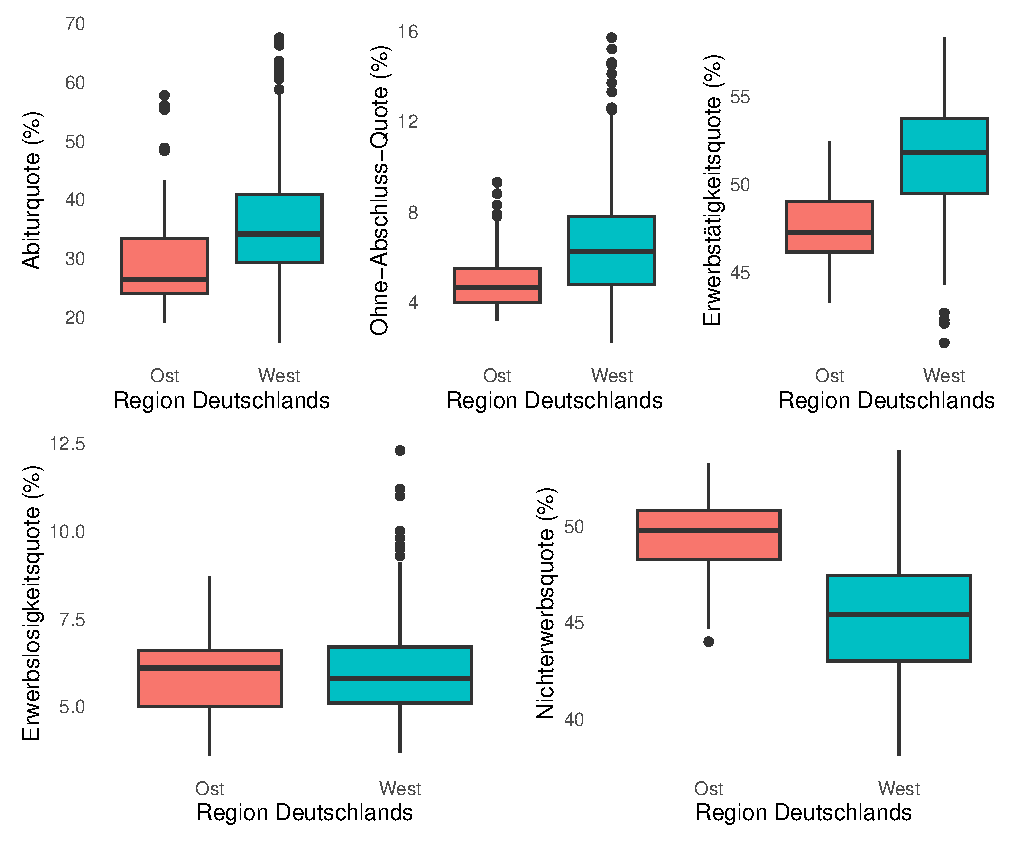
\includegraphics[width=0.5\linewidth]{graphiken/boxplotsoutliers.pdf}
        \vspace{-0.75cm}
        \caption{Kerndichteschätzungen mit Gaußkern für Alter, Größe und Gewicht.}
    \end{figure}
    \begin{lstlisting}
library(ggplot2)
ggplot(df, aes(x = age, y = value)) +
  geom_point() +
  geom_smooth(method = "lm")
    \end{lstlisting}
\end{frame}

% Folie 5 
\begin{frame}[fragile]{R Code Beispiel}
    \frametitle{Unterschiede zwischen Ost- und Westdeutschland}
%    \begin{figure}
%        \centering
%        \includegraphics[width=1\linewidth]{population.pdf}
%        \vspace{-0.75cm}
%        \caption{Kerndichteschätzungen mit Gaußkern für Alter, Größe und Gewicht.}
%    \end{figure}
    \begin{lstlisting}
library(ggplot2)
ggplot(df, aes(x = age, y = value)) +
  geom_point() +
  geom_smooth(method = "lm")
    \end{lstlisting}
\end{frame}

% Folie 6 
\begin{frame}[fragile]{R Code Beispiel}
    \frametitle{Prädiktoren für Arbeitslosigkeit}
    
        \begin{itemize}
            \item Multiples Lineares Modell
        \end{itemize}
    \begin{lstlisting}
model <- lm(Erwerbslos_Quote ~ 
              Abitur_Quote + 
              OhneAbschl_Quote + 
              Erwerbstaetig_Quote,
            data = df2)

summary(model)
    \end{lstlisting}
        \begin{itemize}
            \item Rechts: Ergebnistabelle
        \end{itemize}
\end{frame}


\begin{frame}[fragile]{R Code Beispiel}
    \frametitle{Prädiktoren für Arbeitslosigkeit}
    \begin{figure}
        \centering
        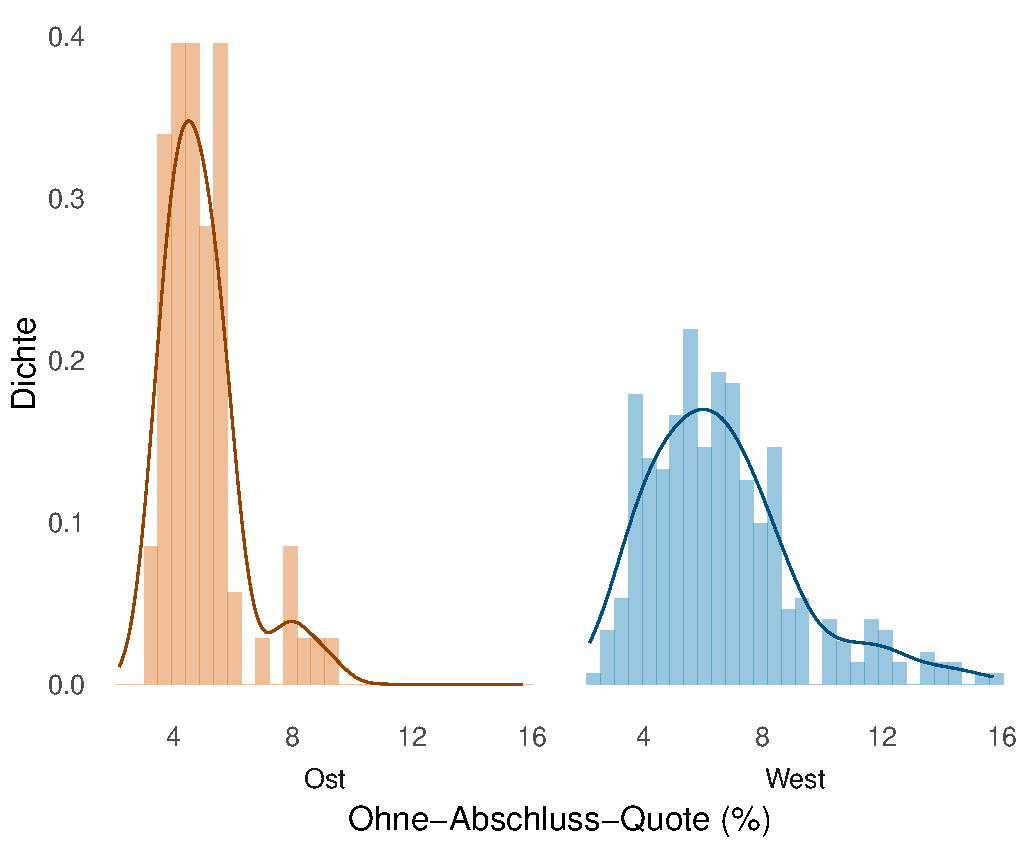
\includegraphics[width=0.2\linewidth]{graphiken/kdeOhneAbschluss.pdf}
        \vspace{-0.75cm}
        \caption{Kerndichteschätzungen mit Gaußkern für Alter, Größe und Gewicht.}
    \end{figure}
    
        \begin{figure}
        \centering
        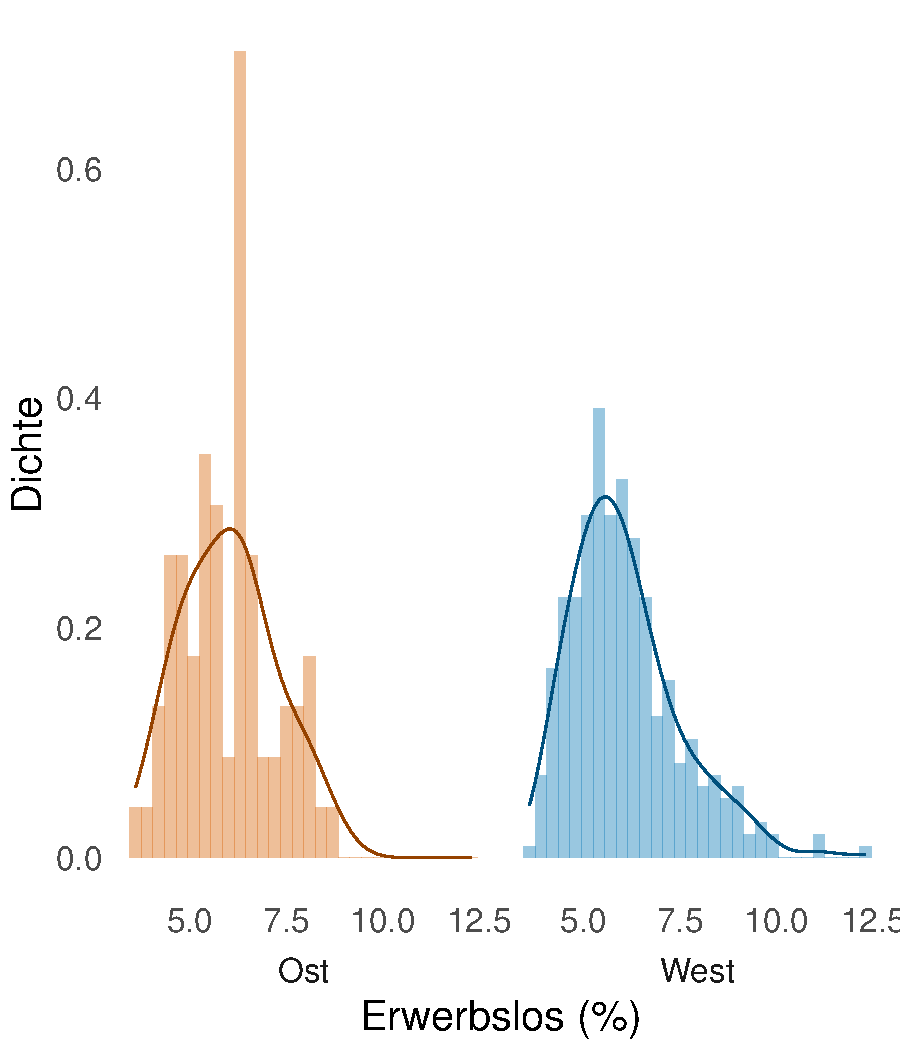
\includegraphics[width=0.2\linewidth]{graphiken/kdeErwerbslos.pdf}
        \vspace{-0.75cm}
        \caption{Kerndichteschätzungen mit Gaußkern für Alter, Größe und Gewicht.}
    \end{figure}

\end{frame}


\begin{frame}[fragile]{R Code Beispiel}
    \frametitle{Prädiktoren für Arbeitslosigkeit}
    \begin{figure}
        \centering
        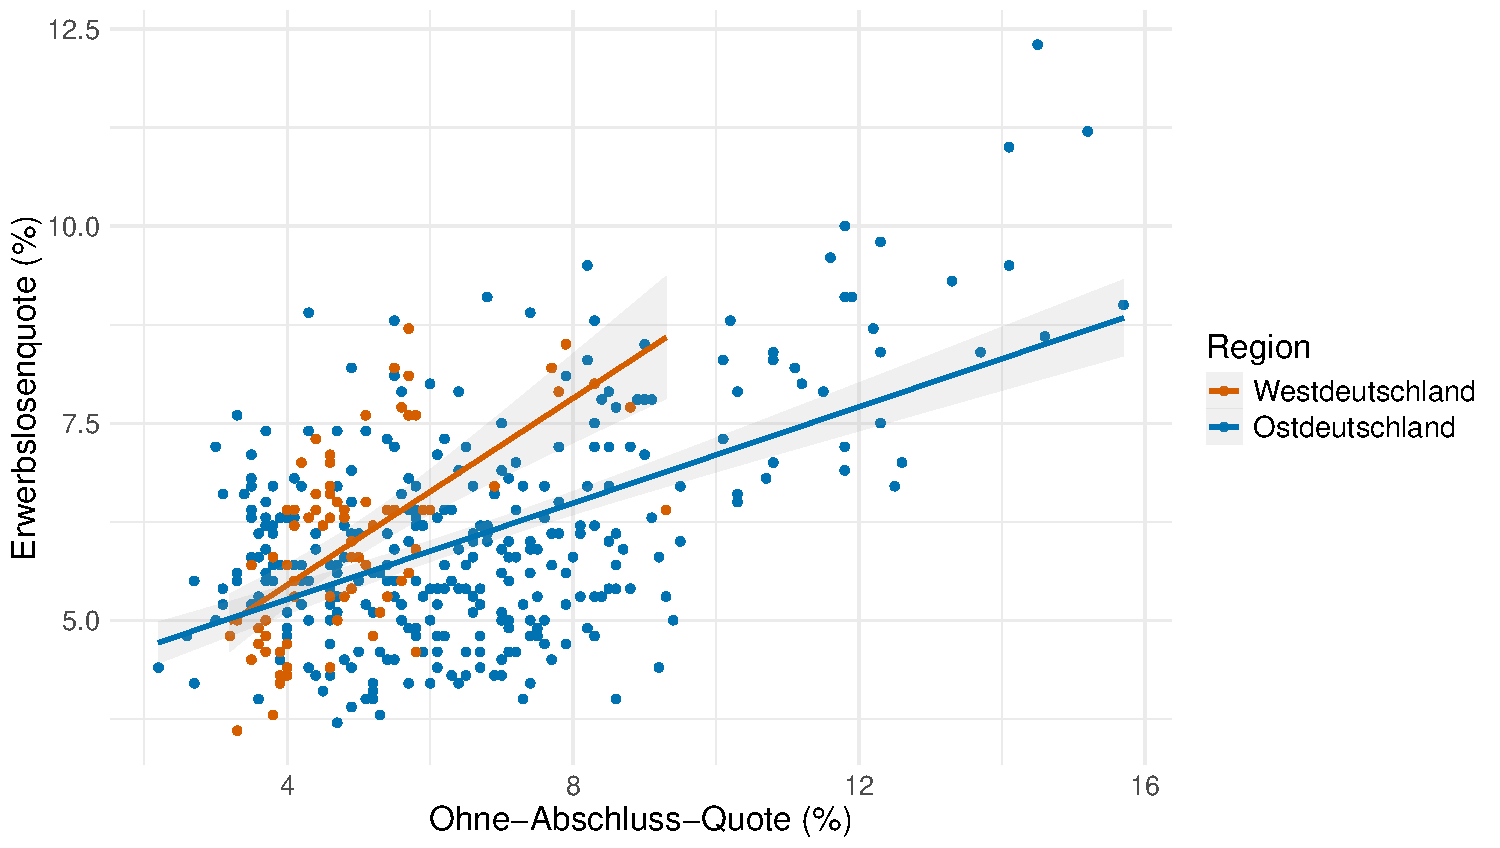
\includegraphics[width=0.5\linewidth]{graphiken/spOhneAbschlussErwerbslos.pdf}
        \vspace{-0.75cm}
        \caption{Kerndichteschätzungen mit Gaußkern für Alter, Größe und Gewicht.}
    \end{figure}

\end{frame}


\begin{frame}[fragile]{R Code Beispiel}
    \frametitle{Pläne für weitere Analysen}
        \begin{itemize}
            \item Hypothesentests (Unterschied zwischen Ost- und West)
            \begin{itemize}
                \item Wilcoxon Test
                \item t-Test
            \end{itemize}
            \item deskriptive Maße
            \begin{itemize}
                \item Median statt Durchschnitt
                \item MAD statt Standardabweichung
            \end{itemize}
        \end{itemize}

\end{frame}



\end{document}
